%\documentclass[pra,showpacs,twocolumn]{revtex4}
%\documentclass[pra,showpacs]{revtex4}
%\documentclass[preprint,showpacs]{revtex4}
\documentclass[10pt,showpacs,twocolumn]{revtex4}
%%%%%%%%%%%%%%%%%%%%%%%%%%%%%%%%%%%%%%%%%%%%%%%%%%%%%%%%%%%%%%%%%%%%%%%%
\usepackage{amssymb}
\usepackage{amsmath}
\usepackage{graphicx}
\usepackage{multirow}
\usepackage{gensymb}
\usepackage{float}
\usepackage{MnSymbol}
\usepackage{gensymb}
\usepackage{comment}


\begin{document}


\title[Scaled ionization cross section of biological molecules]{
Scaled ionization cross section of biological molecules}
\author{A. M. P. Mendez, C. C. Montanari, J. E. Miraglia}
\affiliation{Instituto de Astronom\'{\i}a y F\'{\i}sica del Espacio 
(CONICET--UBA), \\ Buenos Aires, Argentina.}

%\date{\today}% It is always \today, today,

\begin{abstract}
In the present work, we investigate the $Z$ scaling of the cross section 
and impact energy of multicharged ions on molecules of biological 
interest in intermediate to high energy range. 
The cross sections are obtained from distorted--wave calculations (CDW) 
of thirty--six atom--ion collisional systems and the simple 
stoichiometric model (SSM). 
We examine the scaling of seventeen molecules: hydrocarbons, 
DNA and RNA bases, DNA backbone, tetrahydrofuran (THF), and pyrimidines
compounds. 
\end{abstract}

%\keywords{magnetic moment, solar neutrinos, astrophysics}
\pacs{34.50Gb, 34.80Gs, 34.80Dp}

\maketitle
%\ioptwocol

\begin{comment}
\section{Introduction}


%%%%%%%%%%%%%%%%%%%%%%%%%%%%%%%%%%%%%%%%%%%%%%%%%%%%%%%%%%%%%%%%%%%%%%%%
\section{Ionization of Molecules}
\label{sec:molecules}
%%%%%%%%%%%%%%%%%%%%%%%%%%%%%%%%%%%%%%%%%%%%%%%%%%%%%%%%%%%%%%%%%%%%%%%%
%%%%%%%%%%%%%%%%%%%%%%%%%%%%%%%%%%%%%%%%%%%%%%%%%%%%%%%%%%%%%%%%%%%%%%%%


At intermediate impact energies, the $Z^2$ rule no longer holds, and 
other scalings can be considered in this region. For example, the 
molecular cross section and ion impact energy can be reduced with the
projectile charge $Z$, as suggested in in~\cite{janev1980,dubois2013}. 
\end{comment}

\newpage
\begin{figure*}[]
\centering
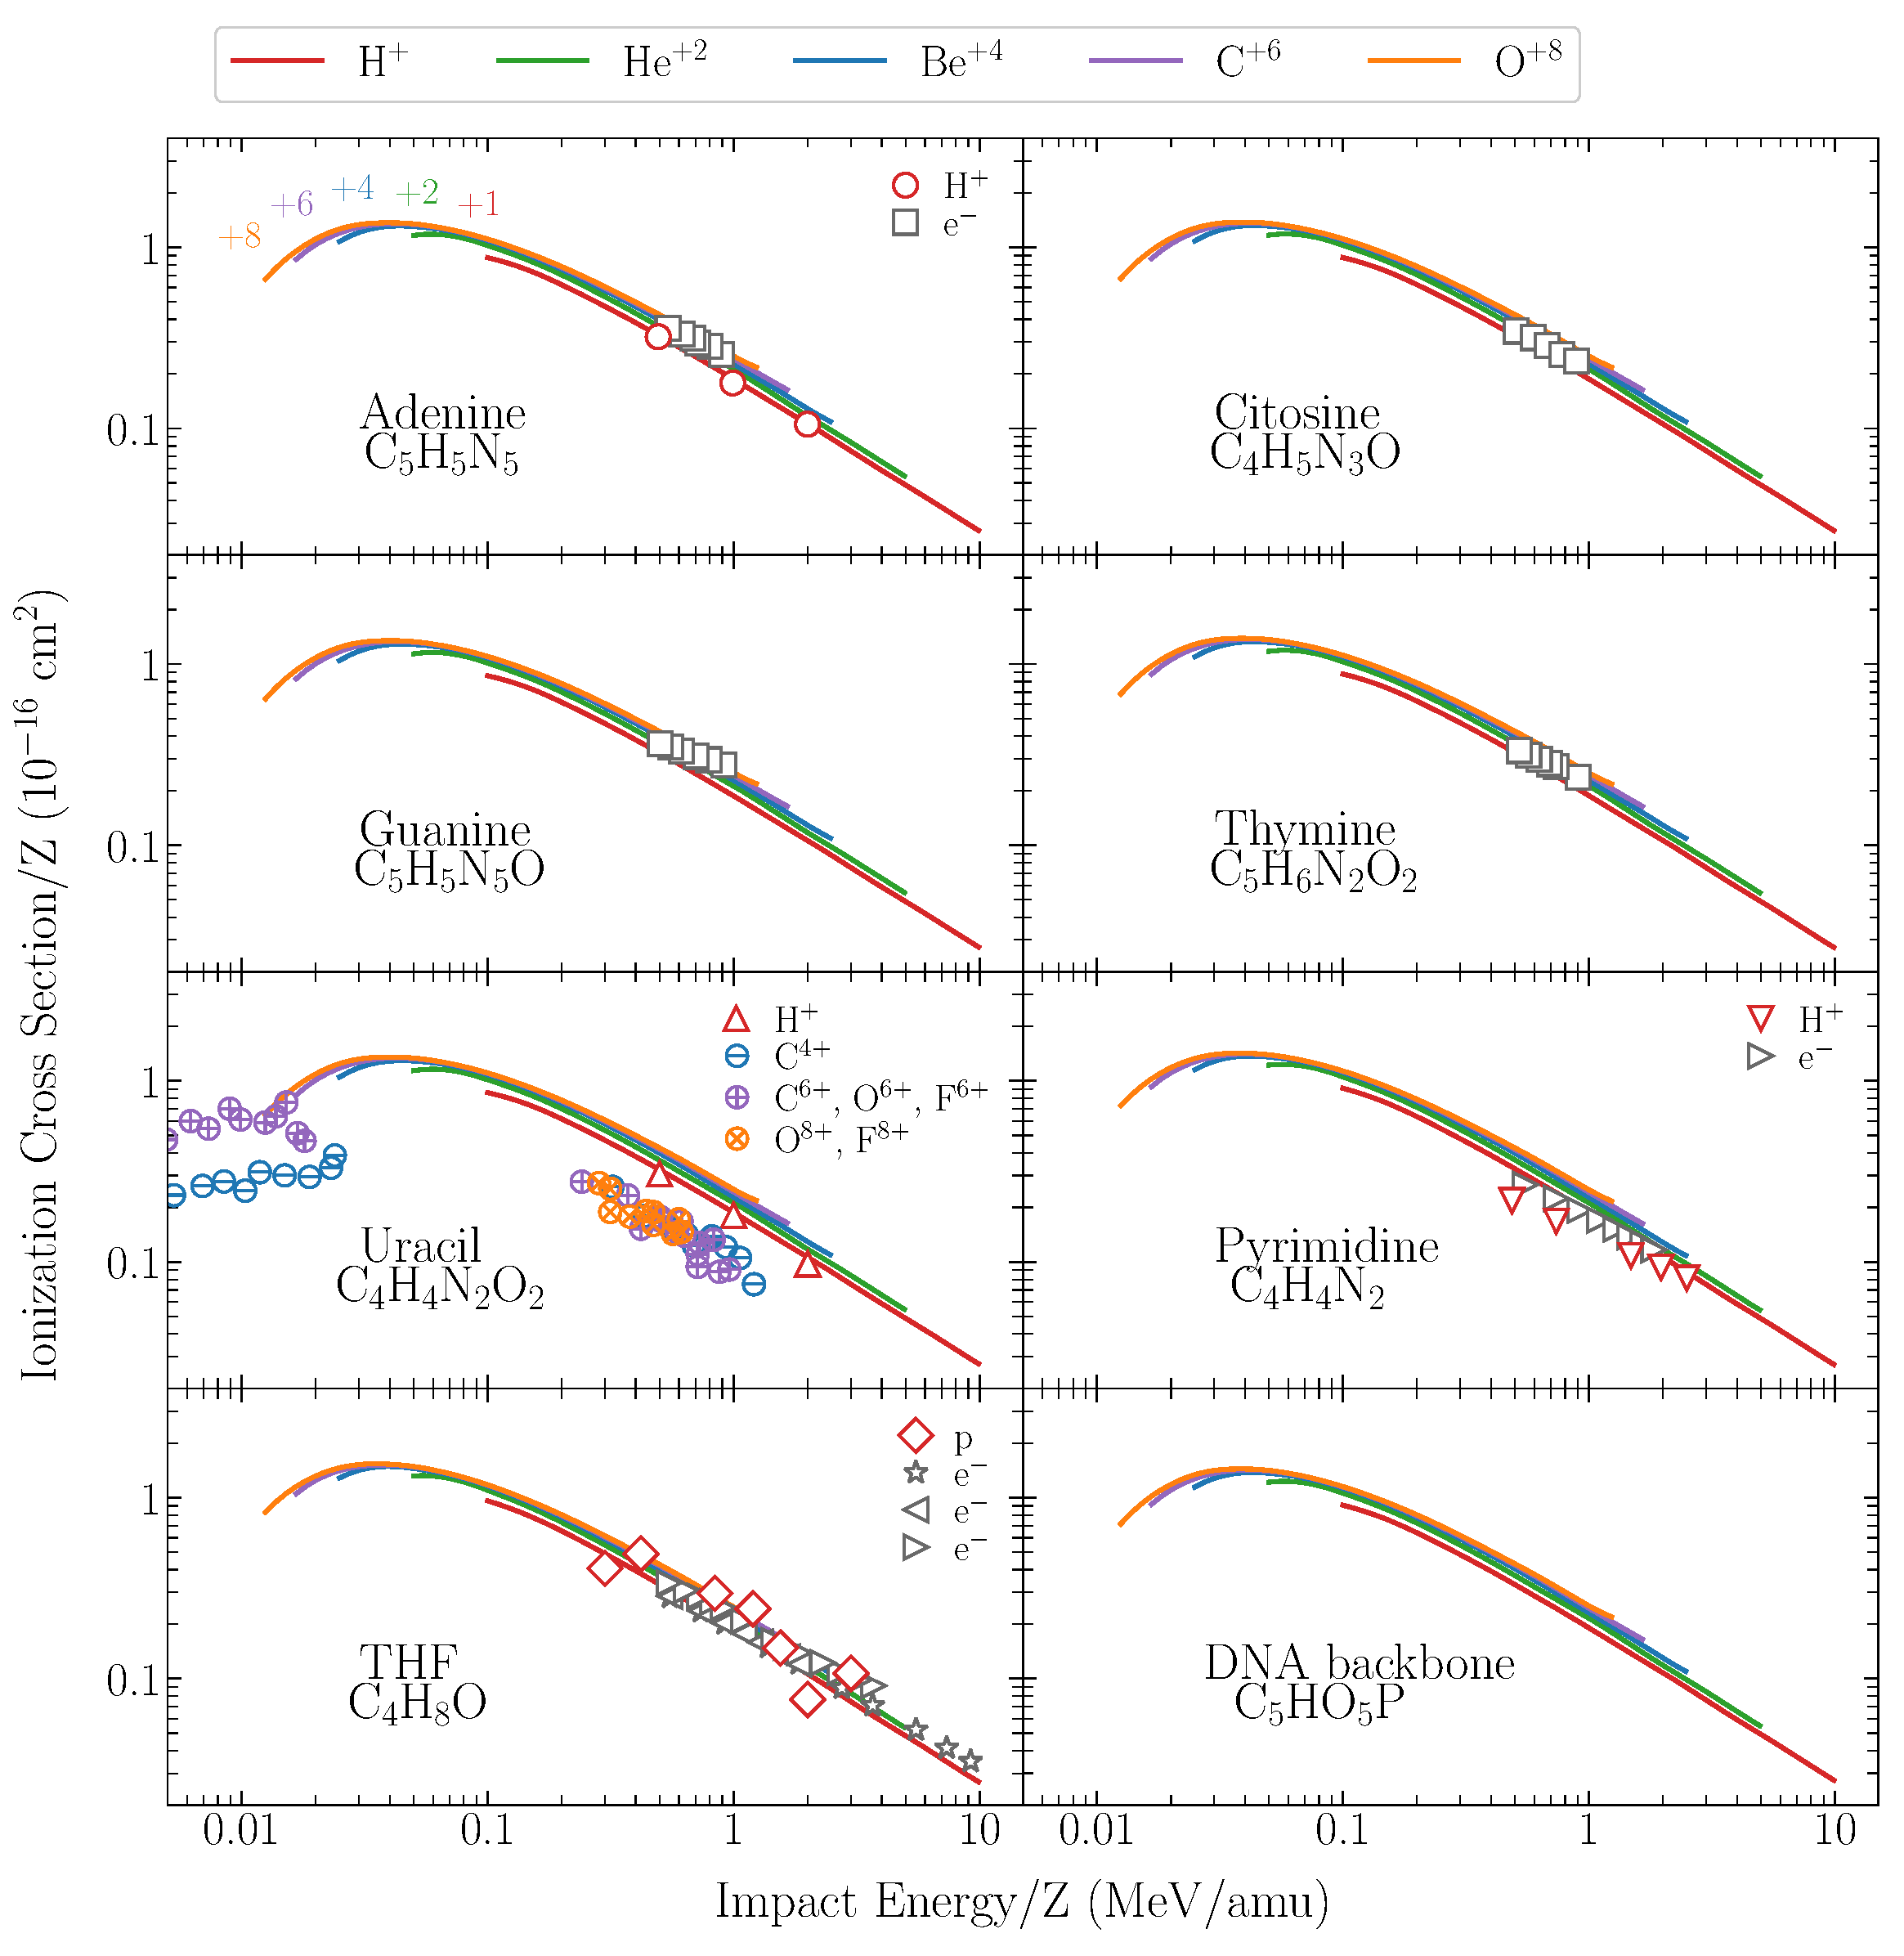
\includegraphics[width=0.8\textwidth]{figuras/zscale.eps}
\caption{Reduced CDW ionization cross section $\sigma_{M}/Z$ as a function 
of ion impact energy $E/Z$. 
Experiments: 
proton impact on 
\mbox{\Large$\circ$} adenine~\cite{iriki2011},
$\triangle$ uracil~\cite{itoh2013}, 
$\bigtriangledown$ pyrimidine~\cite{wolff2014} and 
$\meddiamond$ THF~\cite{wang2016}.
Impact of $\ominus$ C$^{4+}$, 
$\oplus$ C$^{6+}$, O$^{6+}$, F$^{6+}$, and
$\otimes$ O$^{8+}$, F$^{8+}$ on 
uracil~\cite{agnihotri2012,agnihotri2013}. 
Symbols~$\square$~\cite{rahman2016}, $\rhd$~\cite{bug2017}, 
$\lhd$~\cite{wolf2019}, and $\medstar$~\cite{fuss2009} for electron 
impact with equivelocity conversion.}
\label{fig:zreduced}
\end{figure*} 

\begin{figure*}[]
\centering
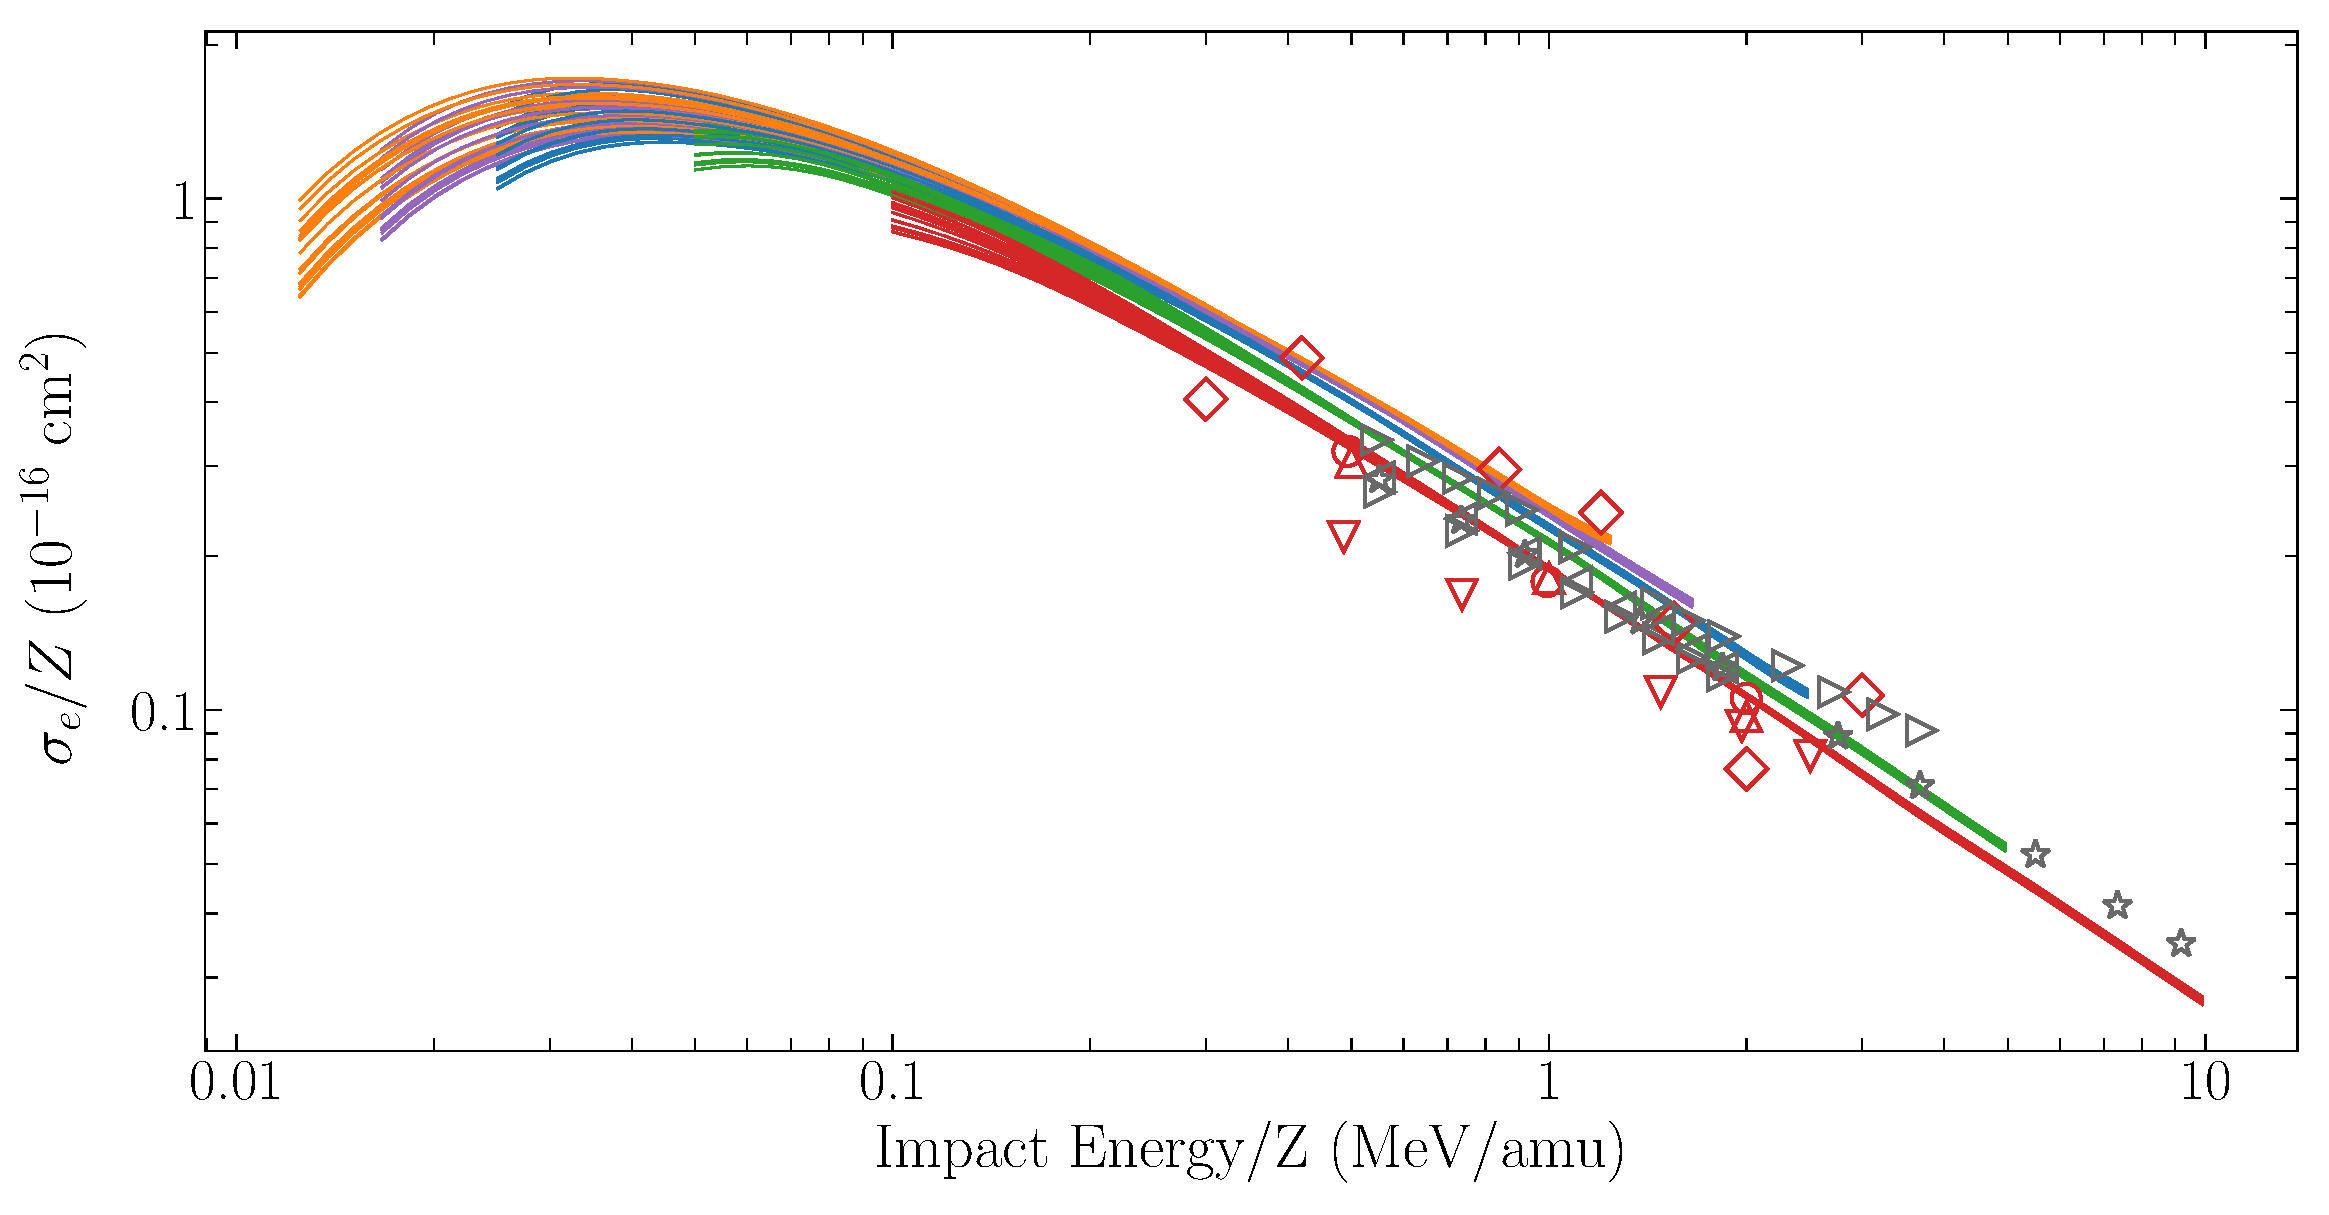
\includegraphics[width=0.8\textwidth]{figuras/zmol85.eps}
\caption{Scaled and reduced ionization cross section per weakly bound 
electron $\sigma_e/Z$ using CDW-based numbers $\nu_{\alpha}^{\text{CDW}}$ 
for molecules listed in Table~1.
Experiments: proton impact on 
\mbox{\Large$\circ$} adenine~\cite{iriki2011}, 
$\triangle$ uracil~\cite{itoh2013}, 
$\bigtriangledown$ pyrimidine~\cite{wolff2014} and $\meddiamond$ 
THF~\cite{wang2016}; electron impact on $\rhd$ pyrimidine~\cite{bug2017},
and $\lhd$, $\medstar$~\cite{wolf2019,fuss2009} THF.}
\label{fig:zredscaled}
\end{figure*}


%%%%%%%%%%%%%%%%%%%%%%%%%%%%%%%%%%%%%%%%%%%%%%%%%%%%%%%%%%%%%%%%%%%%%%%%
%\section{Conclusions}
%%%%%%%%%%%%%%%%%%%%%%%%%%%%%%%%%%%%%%%%%%%%%%%%%%%%%%%%%%%%%%%%%%%%%%%%

\bigskip
%\section*{References}

\begin{thebibliography}{}

\bibitem{iriki2011}
Y. Iriki, Y. Kikuchi, M. Imai, and A. Itoh
Phys. Rev. A \textbf{84}, 052719 (2011).

\bibitem{rahman2016}
M. A. Rahman and E. Krishnakumar,
Electron ionization of DNA bases,
J. Chem. Phys. \textbf{144}, 161102 (2016).

\bibitem{mozejko2003}
P. Mozejko and L. Sanche, 
Radiat Environ. Biophys \textbf{42}, 201 (2003).

\bibitem{tan2018}
H. Q. Tan, Z. Mi, and A. A. Bettiol, 
Phys. Rev. E \textbf{97}, 032403 (2018)

\bibitem{itoh2013} 
A. Itoh, Y. Iriki, M. Imai, C. Champion, and R. D. Rivarola, 
Phys. Rev. A \textbf{88}, 052711 (2013).

\bibitem{agnihotri2012}
A. N. Agnihotri, S. Kasthurirangan, S. Nandi, A.
Kumar, M. E. Galassi, R. D. Rivarola, O. Foj\'{o}n, C. Champion, J. Hanssen,
H. Lekadir, P. F. Weck, and L. C. Tribedi. 
Phys. Rev. A \textbf{85}, 032711 (2012).

\bibitem{agnihotri2013}
A N Agnihotri, S Kasthurirangan, S Nandi, A Kumar, C Champion,, H Lekadir, 
J Hanssen, P FWeck, M E Galassi, R D Rivarola, O Fojon and L C Tribedi, 
J. Phys. B \textbf{46}, 185201 (2013).

\bibitem{champion2012} 
C Champion, M E Galassi, O Foj\'{o}n, H Lekadir, J Hanssen, R D Rivarola,
P F Weck, A N Agnihotri, S Nandi, and L C Tribedi. 
J. Phys.: Conf. Ser. \textbf{373}, 012004 (2012).

\bibitem{wolff2014}
W. Wolff, H. Luna, L. Sigaud, A. C. Tavares, and E. C. Montenegro
J. Chem. Phys. \textbf{140}, 064309 (2014).

\bibitem{bug2017}
M. U. Bug, W. Y. Baek, H. Rabus, C. Villagrasa, S. Meylan, A. B. Rosenfeld,
Rad. Phys. Chem. \textbf{130}, 459--479 (2017).

\bibitem{wang2016}
M. Wang, B. Rudek, D. Bennett, P. de Vera, M. Bug, T. Buhr, W. Y. Baek, 
G. Hilgers, H. Rabus, 
Phys. Rev. A \textbf{93}, 052711 (2016).

\bibitem{wolf2019}
W. Wolff, B. Rudek, L. A. da Silva, G. Hilgers, E. C. Montenegro, 
M. G. P. Homem,
J. Chem. Phys. \textbf{151}, 064304 (2019).

\bibitem{fuss2009}
M. Fuss, A. Muñoz, J. C. Oller, F. Blanco, D. Almeida, P. Limão-Vieira, 
T. P. D. Do, M. J. Brunger, G. Garc\'{i}a,
Phys. Rev. A \textbf{80}, 052709 (2009).

\bibitem{janev1980}
R. K. Janev and L. P. Presnyakov 
J. Phys. B \textbf{13}, 4233 (1980).

\bibitem{dubois2013}
R. D. DuBois, E. C. Montenegro and G. M. Sigaud,
AIP Conference Proceeding \textbf{1525}, 679 (2013).

\begin{comment}


\bibitem{Mohamad2017}
O. Mohamad, B. J. Sishc, J. Saha, A. Pompos, A. Rahimi, M. D. Story, A. J. Davis, D. N. Kim, 
Cancers \textbf{9}, 66 (2017).

\bibitem{galassi2000}
M. E. Galasssi, R. D. Rivarola, M. Beuve, G. H. Olivera and P. D. Fainstein, 
Phys. Rev. A \textbf{62}, 022701 (2000).

\bibitem{ludde2016}
H. J. L\"udde, A. Achenbach, T. Kalkbrenner, H.-C. Jankowiak and T. Kirchner,
Eur. Phys. J. D \textbf{70}, 82 (2016).

\bibitem{ludde2018}
H. J. L\"udde, M. Horbatsch and T. Kirchner,

Eur. Phys. J. B \textbf{91}, 99 (2018).

\bibitem{fainstein1988}
Fainstein P.D., Ponce V. H. and Rivarola R. D. 
J. Phys. B: At. Mol. Opt. Phys. \textbf{21} 287 (1988).


\bibitem{miraglia2008} 
J. E. Miraglia and M. S. Gravielle. 
Phys Rev A \textbf{78}, 052705 (2008)

\bibitem{miraglia2009} 
J. E. Miraglia, 

Phys. Rev. A \textbf{79}, 022708 (2009).

\bibitem{Denifl2011}
Denifl S., Märk T.D., Scheier P. 
The Role of Secondary Electrons in Radiation Damage. 
In Radiation Damage in Biomolecular Systems. Biological and Medical Physics, Biomedical Engineering. 
Eds: García Gómez-Tejedor G., Fuss M. 
Springer, Dordrecht (2012) 

\bibitem{toburen1975} 
W. E. Wilson and L. H. Toburen. 
Phys. Rev. A \textbf{11}, 1303 (1975).

\bibitem{toburen1976} 
D. J. Lynch, L. H. Toburen, and W. E. Wilson. 
J. Chem. Phys. \textbf{64}, 2616 (1976).

\bibitem{gamess}

M. W. Schmidt, K. K. Baldridge, J. A. Boatz, S. T. Elbert, M. S. Gordon, 
J. H. Jensen, S. Koseki, N. Matsunaga, K. A. Nguyen, S. J. Su, T. L. Windus, 
M. Dupuis, J. A. Montgomery 
J. Comput. Chem. \textbf{14}, 1347-1363 (1993).

\bibitem{salvat1995}
Salvat, F., Fern\'andez-Varea, J.M., Williamson, W.
Comput. Phys. Commun. \textbf{90}, 151--168 (1995)

\bibitem{mendez2016} 
A.M.P. Mendez, D.M. Mitnik, and J.E. Miraglia.
Int. J. Quantum Chem. \textbf{24} ,116 (2016).

\bibitem{mendez2018} 
A.M.P. Mendez, D.M. Mitnik, and J.E. Miraglia. 
Adv. Quant. Chem. \textbf{76}, 117--132 (2018).

\bibitem{montanari2017} 

C. C. Montanari, J. E. Miraglia,
Nucl. Instr. Meth. Phys. Res. B \textbf{407}, 236--243 (2017).

\bibitem{miraglia2019} 
J. E. Miraglia,
O$^{8+}$ on H, C, N, O, P, and S atoms (to be published).


\bibitem{surdutovic2018} 
E. Surdutovich and A. V. Solov'yov, 
arXiv:1312.0897v, (2013)

\bibitem{abril2015} 
P. de Vera, I. Abril, R. Garcia-Molina and A. V. Solov'yov,
Journal of Physics: Conference Series \textbf{438}, 012015 (2013).

\bibitem{Rudd1992} 
M. E. Rudd, Y.-K. Kim,, D. H. Madison and T. J. Gay.
Rev. Mod. Phys. \textbf{64}, 44--490 (1992).

\bibitem{lynch1976}
D. J. Lynch, L. H. Toburen, and W. E. Wilson,
J. Chem. Phys. \textbf{64}, 2616 (1976).

\bibitem{rudd1985}
M.E. Rudd, Y.-K. Kim, D.H. Madison, J.W. Gallagher,
Review of Modern Physics, \textbf{57}, 965--994 (1985).

\bibitem{luna2007}
H. Luna, A. L. F. de Barros, J. A. Wyer, S. W. J. Scully, J. Lecointre, 
P. M. Y. Garcia, G. M. Sigaud, A. C. F. Santos, V. Senthil, M. B. Shah, 
C. J. Latimer, and E. C. Montenegro,
Phys. Rev. A \textbf{75}, 042711 (2007).

\bibitem{ludde2019}
H J L\"udde {\it et al.} 2019 
J. Phys. B: At. Mol. Opt. Phys. in press 
https://doi.org/10.1088/1361-6455/ab3a63

\bibitem{Hush}
Hush, N.S.; Cheung, A.S., 
Chem. Phys. Lett., \textbf{34}, 11 (1975).

\bibitem{Verkin}
Verkin, B.I.; Sukodub, L.F.; Yanson, I.K., 

\bibitem{Dougherty}
Dougherty, D.; Younathan, E.S.; Voll, R.; Abdulnur, S.; McGlynn, S.P., 
J. Electron Spectrosc. Relat. Phenom., \textbf{13}, 379 (1978).

\bibitem{lee2003} 
Jung-Goo Lee, Ho Young Jeong, and Hosull Lee, Charges of
Bull. Korean Chem. Soc. \textbf{24}, 369 (2003).

\bibitem{rappe1991} 
A. K. Rappe, A. K.and W. A. Goddard III,. 
J. Phys. Chem. \textbf{95}, 3358 (1991).
\end{comment}

\end{thebibliography}

\end{document}
